\section{Design Methodologies}
System design is the process of developing specifications for a candidate system that meet the criteria established in the system analysis. Major step in the system design is the preparation of the input forms and the output reports in a form applicable to the user.
\newline
The main objective of the system design is to use the package easily by any computer operator. System design is the creative act of invention, developing new inputs, a database, offline files, method, procedures and output for processing business to meet an organization objective. System design builds information gathered during the system analysis.
\newline
In design an efficient and effective system is of great importance to consider the human factor and equipment that these will require to use. System analyst must evaluate the capabilities and limitations of the personal and corresponding factors of the equipment itself. The characteristics associated with effective system operation are reaccessibility, decision making ability, economy, flexibility, reliability and simplicity.
\newline
We have followed the waterfall model. It is the simplest process model which states that the phases are organized in linear order. One of the main advantages of the model is its simplicity. It is conceptually straight forward and divide the large task of building a software system into a series of cleanly divided phases.
\newline
Waterfall model is the most widely used process model. It is well suited for routine type of projects where the requirements are well understood. That is, if developing organization is quite familiar with the problem domain and the requirements for the software are quite clear, the water fall model works well.
\subsection*{Input design}
Input design is the process of converting the user inputs to a computer-based format. The design for handling input specifies how data are accepted for computer processing. Input design is a part of overall system design that needs careful attention and if includes specifying the means which action are taken. A system user interacting through a workstation must be able to tell the system whether to accept input ,produce a report or end processing. The collection of input data is considered to be the most extensive part of the system design. The major activities carried out are:

\begin{itemize}
\item Collection of needed data from the source.
\item Conversion of data into computer accepted.
\item Verification of converted data.
\item Checking data for accuracy.
\item To ensure that input is understood by and acceptable to the user.
\end{itemize}

\subsection*{Output design}
The output design has done so that the results of processing should be communicated to the user. Effective output design will improve the clarity and performance of outputs. Output is the main reason for developing the system and the basis on which they will evaluate the usefulness of the application.
\newline
Output design phase of the system is concerned with the convergence of information to the end user-friendly manner. The output design should be efficient, intelligible so that the system relationship with the end user is improved and they‟re by enhancing the process of decision making.
Output design objectives

\begin{itemize}
\item It provides maximum information to the user according to their needs.
\item Outputs were identified and described.
 \itemProvides convenient and predicted output to the user.
\end{itemize}
The first part of our output is the detected laser spot being circled in the cam window
\section{System Architecture}
A system architecture can comprise system components that will work together to implement the overall system. 
A system architecture is a conceptual model that defines the structure, behavior, and more views of a system. An architecture description is a formal description and representation of a system, organized in a way that 
supports reasoning about the structures and behaviors of the system.
\newline
In the system architecture of AURO, the main component is the AURO API. It is the only component which is performing all the operations.  Input is accepted from the user through the AURO window. User can input the query using any device that has internet access.
\newline
Query or the input is accepted only in English language and the answer or output will be displayed after searching for it in the databases used such as Google & Wikipedia, in the same AURO window. No more components are involved here.
\vspace{1cm}
\begin{figure}[!h]
  \hspace{.3cm}
  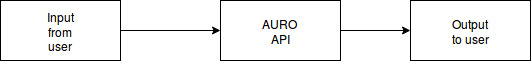
\includegraphics[width=.9\textwidth]{archt.jpg} 
  \caption{Architecture for Auro}
  \label{fig:archt}
\end{figure}

%\newpage
\section{Data Flow Diagram}
A data flow diagram (DFD) is a graphical representation of the flow of data through a system. A DFD is often used as a preliminary step to create an overview of the system without going into detail. It is used in the problem analysis. It views system as a function that atrnsforms input into the desired outputs. The data undergoes a series of transformations before it becomes the output. The data flow diagram aims to capture transformations that take place within the system to the input data so that eventually the output is produced. The agent that performs the transformation is the process. So, a DFD shows the movement of data through different processes or transformations in the system.

\subsection*{Level 0 Data Flow Diagram}
The level 0 data flow diagram shown in Figure \ref{fig:level0} contain an entity, user and the main process of the system. The user provide commands in the form of text. These commands are then converted into natural language. Further it search the database for the corresponding answer. The system retrieves the answer to user as final result.  
\begin{center}

\begin{figure}[!h]
  \hspace{2cm}
  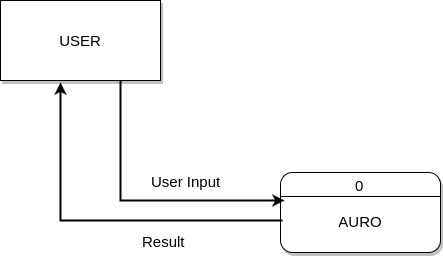
\includegraphics[width=.7\textwidth]{level0.jpg} 
  \caption{Level 0 DFD}
  \label{fig:level0}
\end{figure}
\end{center}

\subsection*{Level 1 Data Flow Diagram}
A level 1 DFD represents the system's major process, data flows and the data stores at a high level of detail.The level 1 DFD shown in Figure \ref{fig:level1} contain one external entity the user. The text command provided by the user is tokenized into words which forms group of words. From this group, the required keywords are filtered neccessary for searching the datbase. The system search database for the corresponding answer and is given to the user as the final result.
\begin{figure}[!h]
  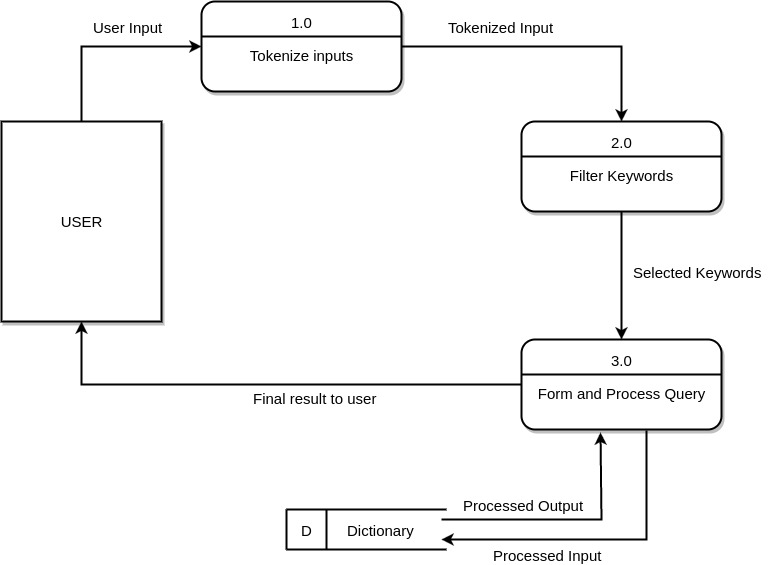
\includegraphics[width=1\textwidth]{level1.jpg}
  \caption{Level 1 DFD}
  \label{fig:level1}
\end{figure}


\newpage
\section{Use Case Diagram}
A use case diagram shown in Figure \ref{fig:usecase} is the represention  of the user's interaction with the system that shows the relationship between the user and the different use cases. The use case diagrams are also referred to as behaviour diagrams used to describe a set of actions (use cases) that some systems or should or can perform in collaboration with one or more external users of the system. Each use case should provide some observable and valuable result to the stakeholders of the system.
\newline
External entities are reffered to as actors which can be human users, external hardware or other systems. An actor is a named stick figure, or a class rectangle with $<<$actor$>>$  keyword. A use case is a single unit of meaningful work.The purpose of the use case diagrams is simply to provide the high level view of the system and convey the requirements. The use case is denoted by an ellipse.
\newline
The use case diagram of AURO consist of one external entity the user and four use cases, user input, processing the text, search datbase and display the result. The user provide input to the system which is processed into natural language by the use case processing the text.  
\begin{figure}[!h]
  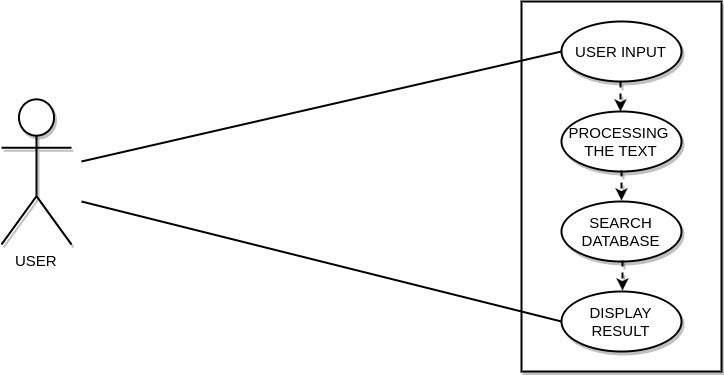
\includegraphics[width=1\textwidth]{usecase.jpg}
  \caption{Use Case Digram}
  \label{fig:usecase}
\end{figure}

